% Document
\documentclass[12pt, a4paper]{article}
\usepackage[T1]{fontenc}
\usepackage[utf8]{inputenc}
\usepackage{authblk}
\usepackage{lipsum}
\usepackage{hyperref}

% Figure and table formating
\usepackage{epsfig}
\usepackage{tabu}
\usepackage{rotating}
\usepackage{pbox}
\usepackage{framed, multicol}
\usepackage[framemethod=TikZ]{mdframed}
\usepackage{float}
\usepackage[left=1.25 in, right=1.25 in, top=1.25 in, bottom=1.25 in]{geometry}

% Fonts - Mathtime
%\usepackage{txfonts}
\usepackage{amsmath} % Add amssymb if not using Mathtime

% Text
\setlength{\parindent}{0.5in}
\frenchspacing  \tolerance = 800  \hyphenpenalty = 800

\usepackage{lineno} % Line numbers
\def\linenumberfont{\normalfont\footnotesize\ttfamily}
\setlength\linenumbersep{0.2 in}

\usepackage{setspace}

% Format section and subsection headers
\makeatletter
\renewcommand{\section}{\@startsection
{section}%                   % the name
{1}%                         % the level
{0mm}%                       % the indent
{-\baselineskip}%            % the before skip
{0.5\baselineskip}%          % the after skip
{\normalfont\bf\large}} % the style

\renewcommand{\subsection}{\@startsection
{subsection}%                   % the name
{2}%                         % the level
{0mm}%                       % the indent
{-\baselineskip}%            % the before skip
{0.5\baselineskip}%          % the after skip
{\normalfont\bf}} % the style
\makeatother

% Other
\usepackage{graphicx}
\usepackage[singlelinecheck=false,font=small,labelfont=bf]{caption}

% Bibliography
\usepackage[numbers, compress]{natbib} % Bibliography - APA
\bibpunct{(}{)}{;}{a}{}{,}

% Format the Bibliography appropriately
% increase \bibhang to take care of the numbers
\setlength{\bibhang}{0pc}
\makeatletter
% patch \@lbibitem to print the current number before the authors
\patchcmd{\@lbibitem}
  {]}
  {] \theNAT@ctr. \newline }
  {}{}
\makeatother


%%%%%% FRONT MATTER %%%%%%%%%

\begin{document}
\renewcommand\thefigure{S\arabic{figure}}

\begin{figure}

    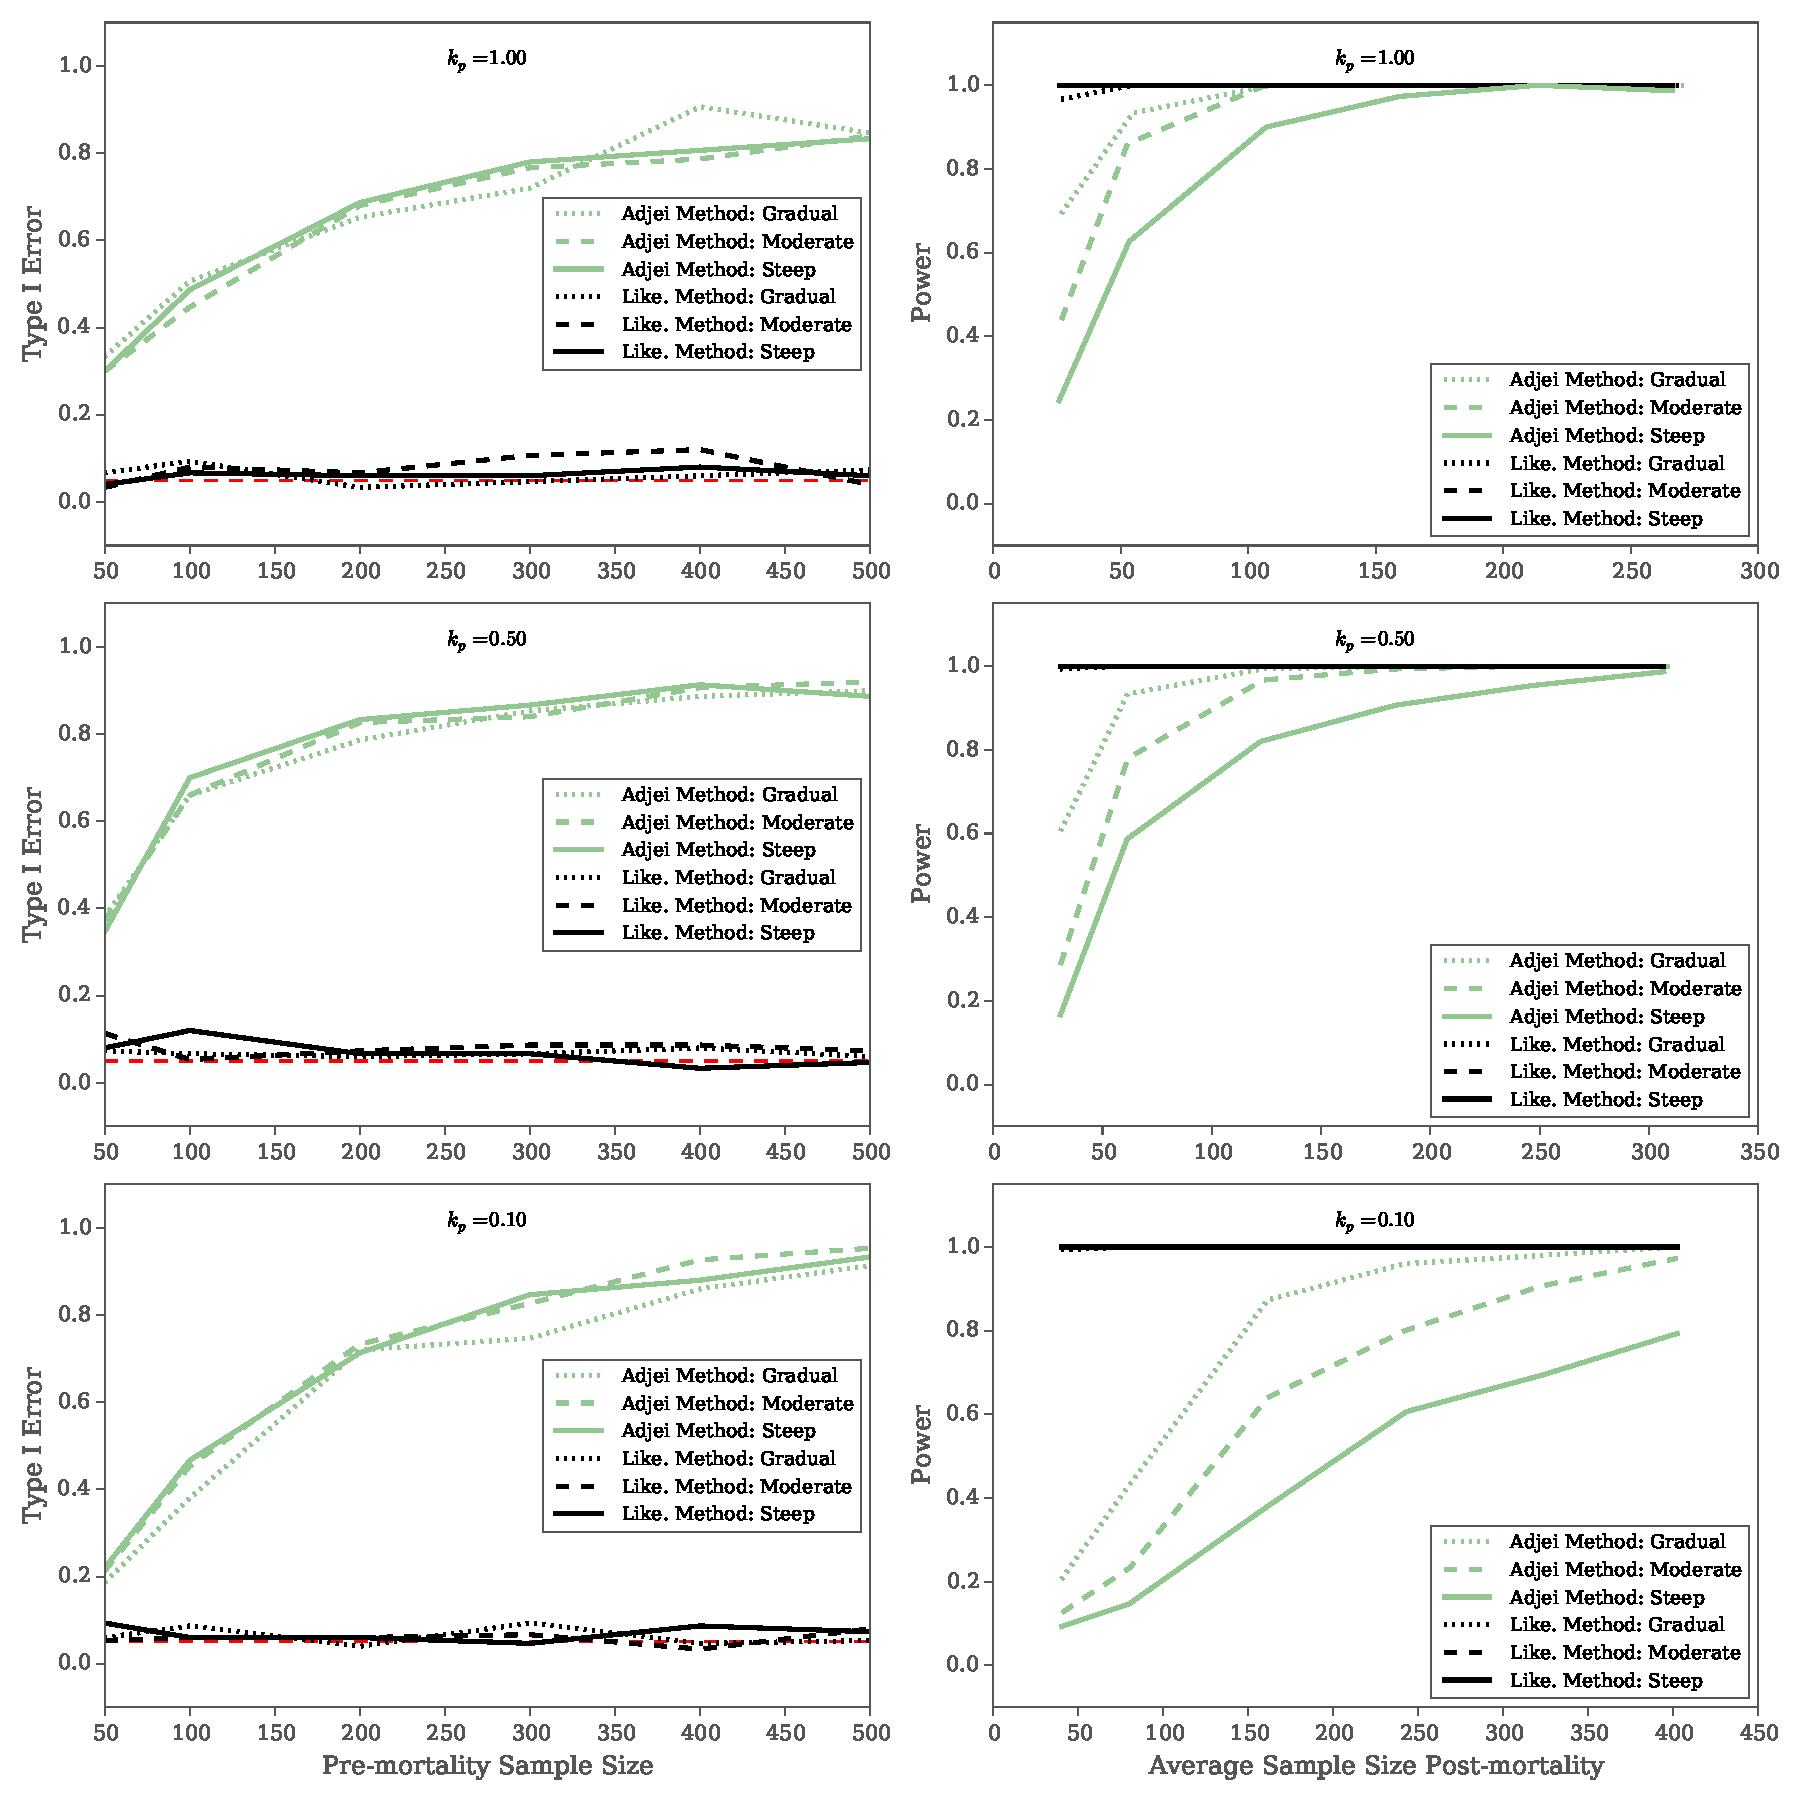
\includegraphics[width=\textwidth]{/Users/mqwilber/Repos/parasite_mortality/results/typeIpower_figure_for_mu10}

    \captionsetup{justification=centering, singlelinecheck=false}
    \caption*{\textbf{Supplementary Fig. S1}}
    %\caption{\doublespacing The type I error rate and the power of the Likelihood Method (black lines) and the Adjei Method (green lines) when $\mu_p = 10$ for various shapes of the host survival function and levels of aggregation $k_p$.  The first column gives the type I error rate of each method for falsely detecting PIHM when none is present.  The red line gives the the pre-set type I error rate of $\alpha = 0.05$.  The second column gives the power of a given method to detect PIHM when it is actually occurring. }
    \label{fig:typeI10}

\end{figure}

\begin{figure}

    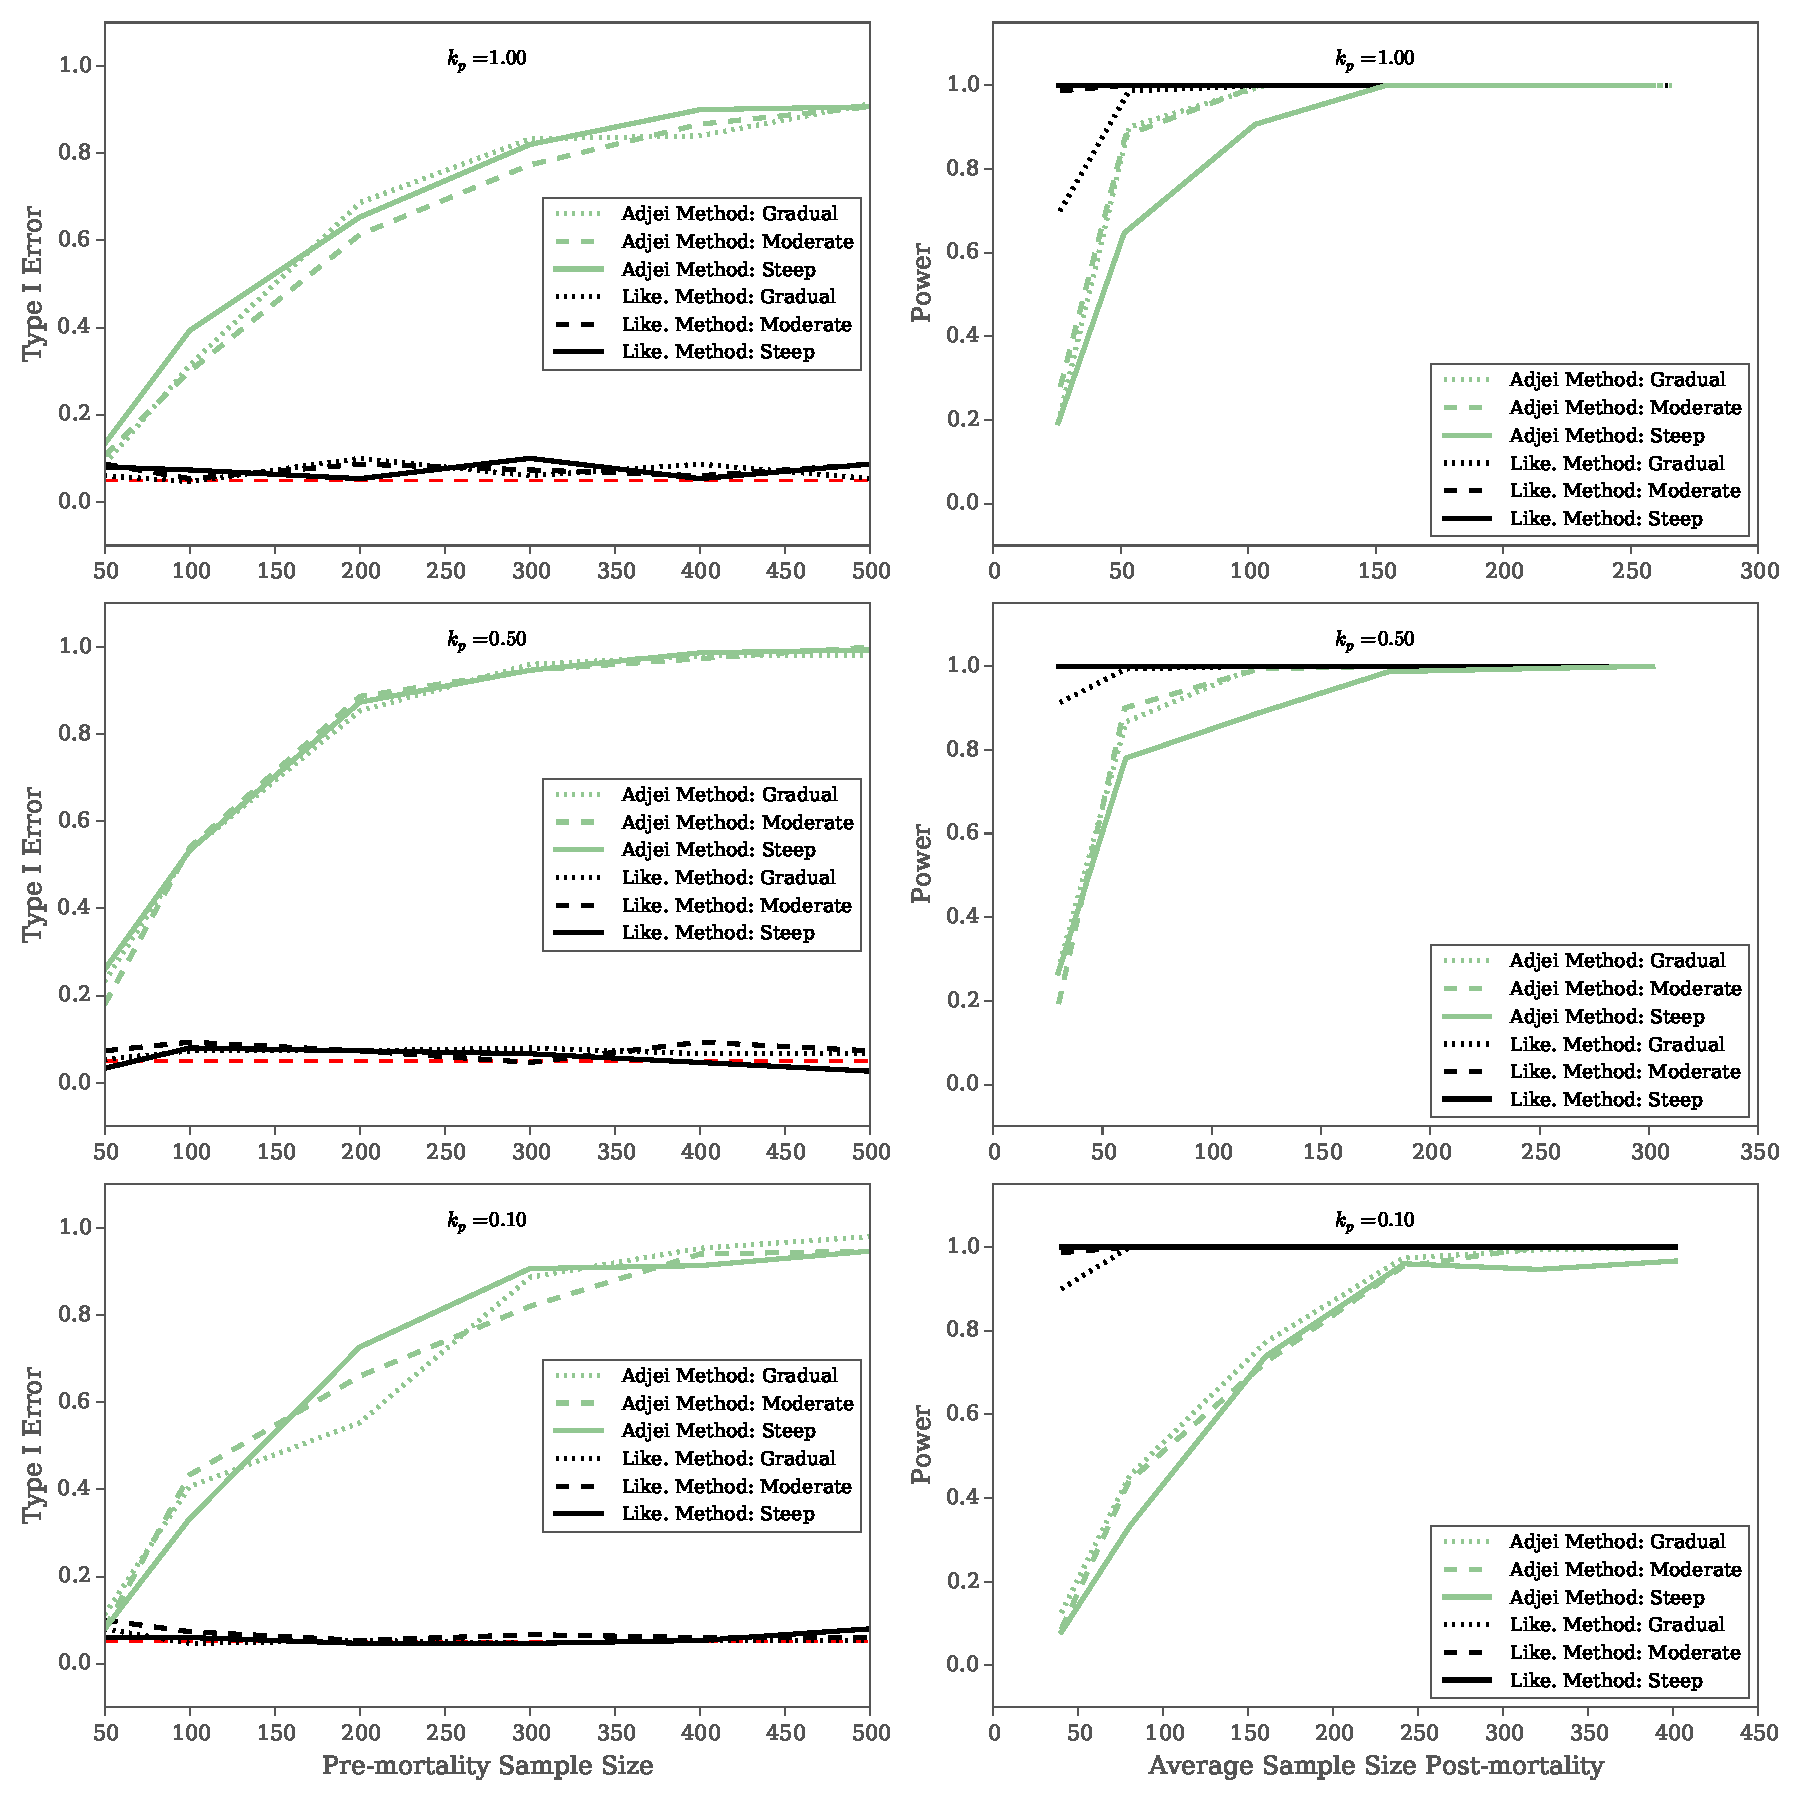
\includegraphics[width=\textwidth]{/Users/mqwilber/Repos/parasite_mortality/results/typeIpower_figure_for_mu50}

    \captionsetup{justification=centering, singlelinecheck=false}

    \caption*{\textbf{Supplementary Fig. S2}}
    %\caption{\doublespacing The type I error rate and the power of the Likelihood Method (black lines) and the Adjei Method (green lines) when $\mu_p = 50$ for various shapes of the host survival function and levels of aggregation $k_p$.  The first column gives the type I error rate of each method for falsely detecting PIHM when none is present.  The red line gives the the pre-set type I error rate of $\alpha = 0.05$.  The second column gives the power of a given method to detect PIHM when it is actually occurring. }
    \label{fig:typeI50}

\end{figure}

\begin{figure}

    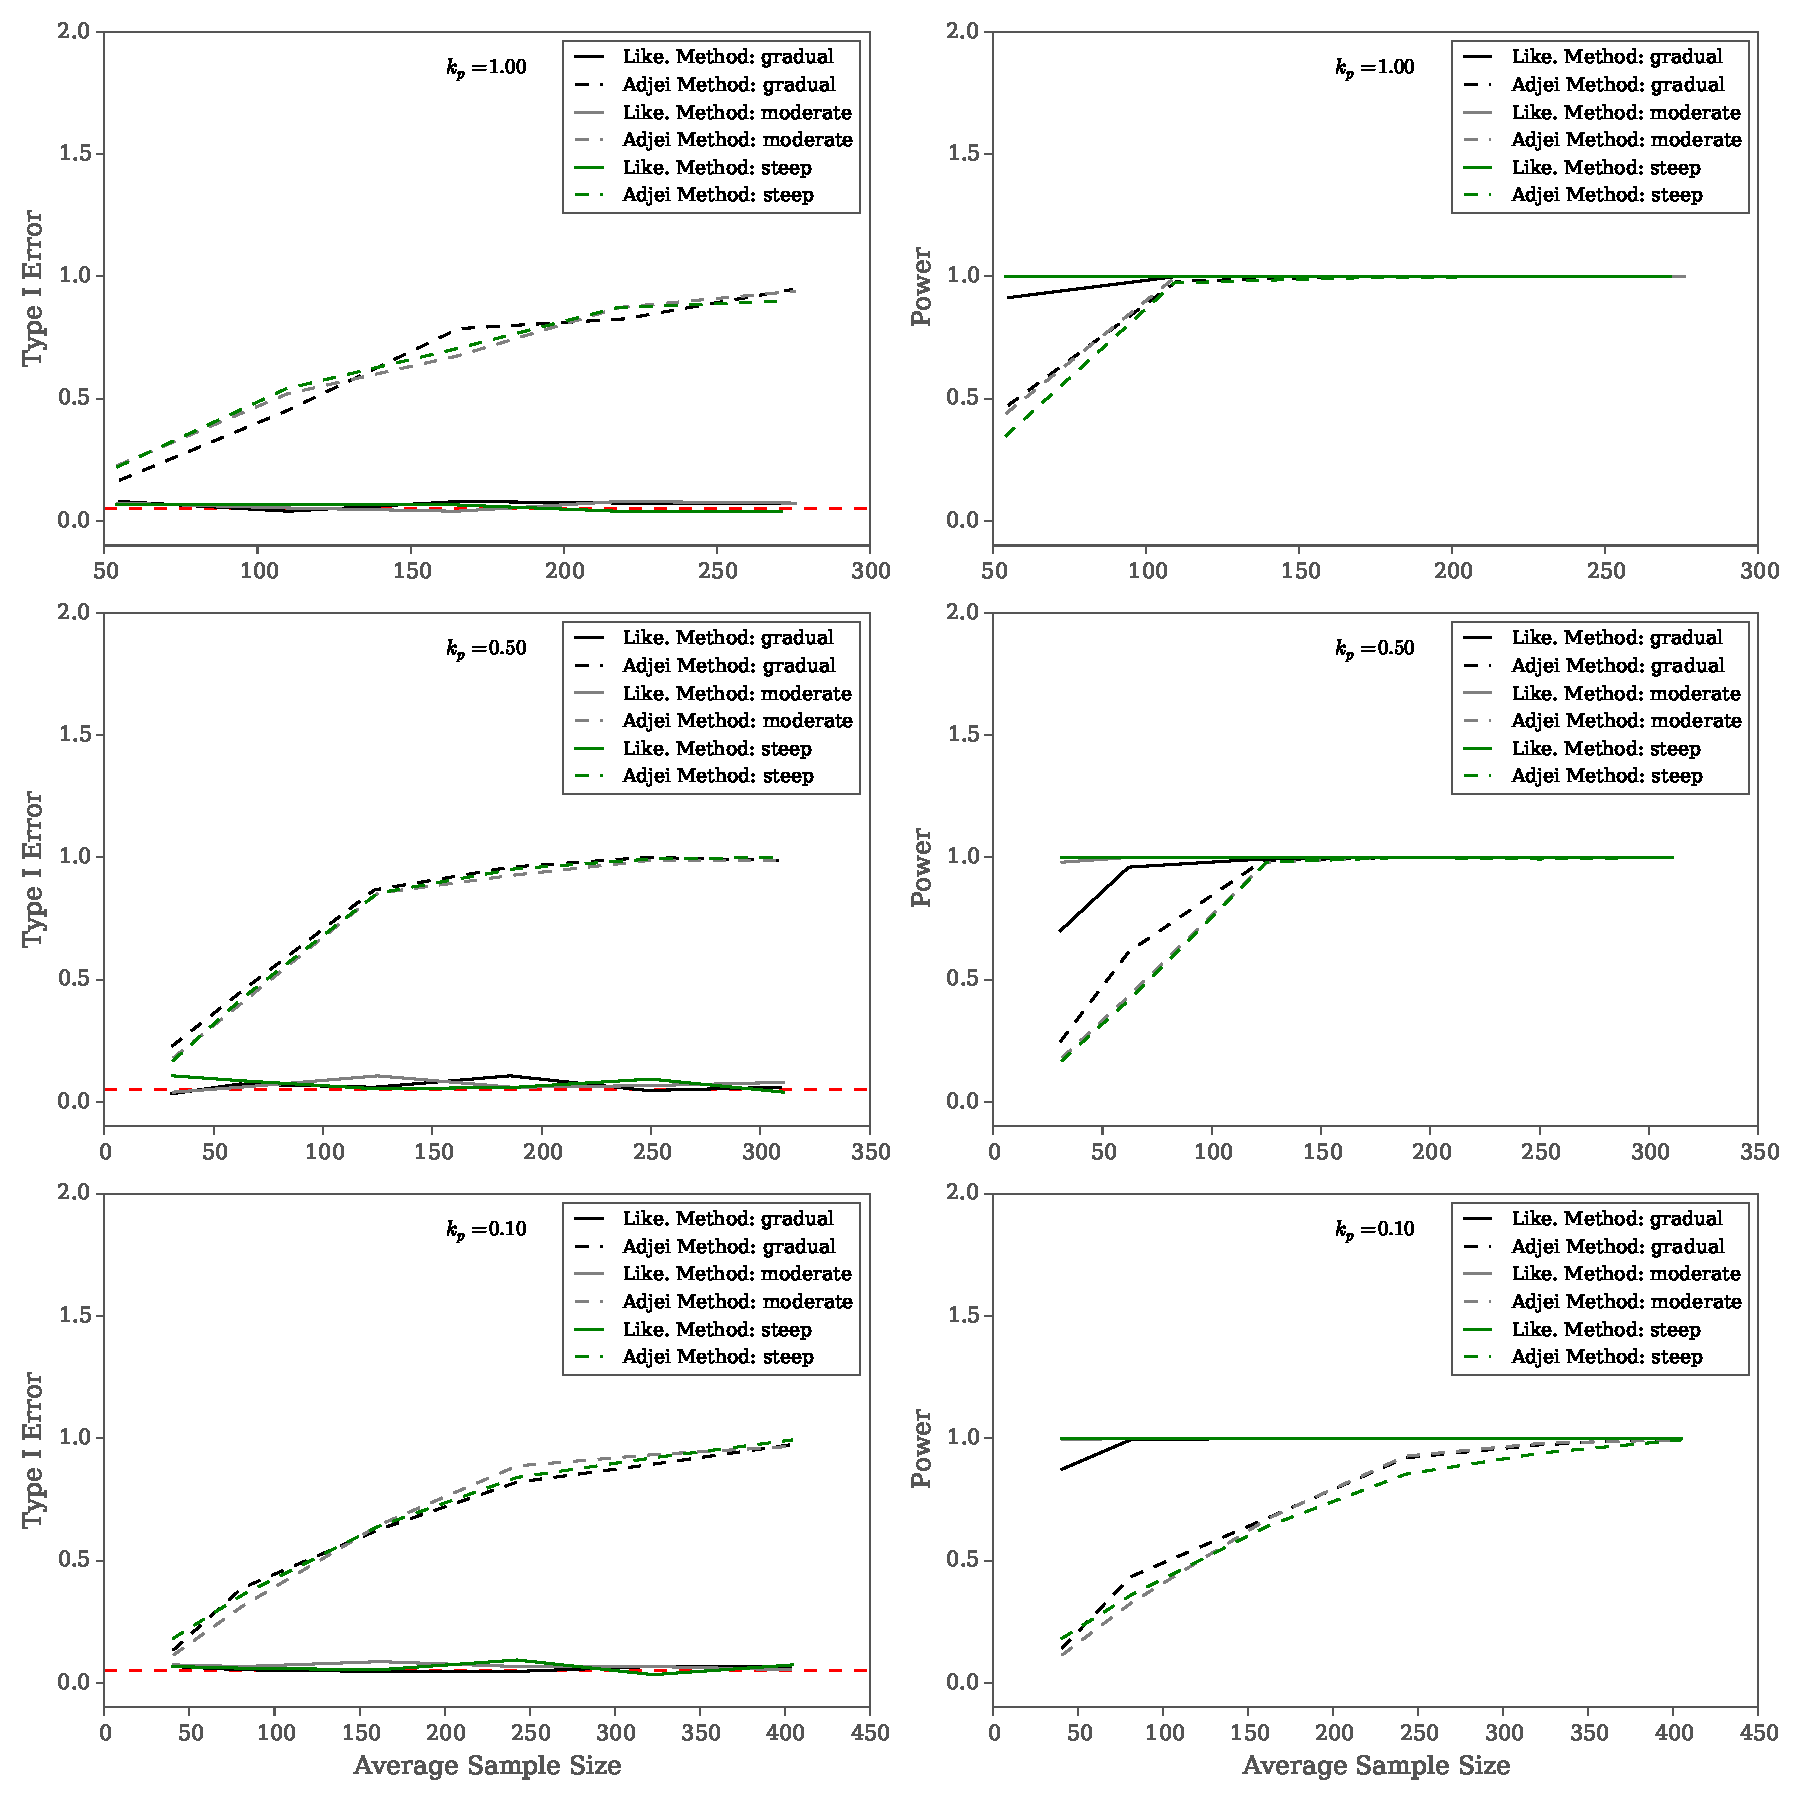
\includegraphics[width=\textwidth]{/Users/mqwilber/Repos/parasite_mortality/results/typeIpower_figure_for_mu100}

    \captionsetup{justification=centering, singlelinecheck=false}

    \caption*{\textbf{Supplementary Fig. S3}}

    %\caption{\doublespacing The type I error rate and the power of the Likelihood Method (black lines) and the Adjei Method (green lines) when $\mu_p = 100$ for various shapes of the host survival function and levels of aggregation $k_p$.  The first column gives the type I error rate of each method for falsely detecting PIHM when none is present.  The red line gives the the pre-set type I error rate of $\alpha = 0.05$.  The second column gives the power of a given method to detect PIHM when it is actually occurring. }
    \label{fig:typeI100}

\end{figure}

\begin{figure}

    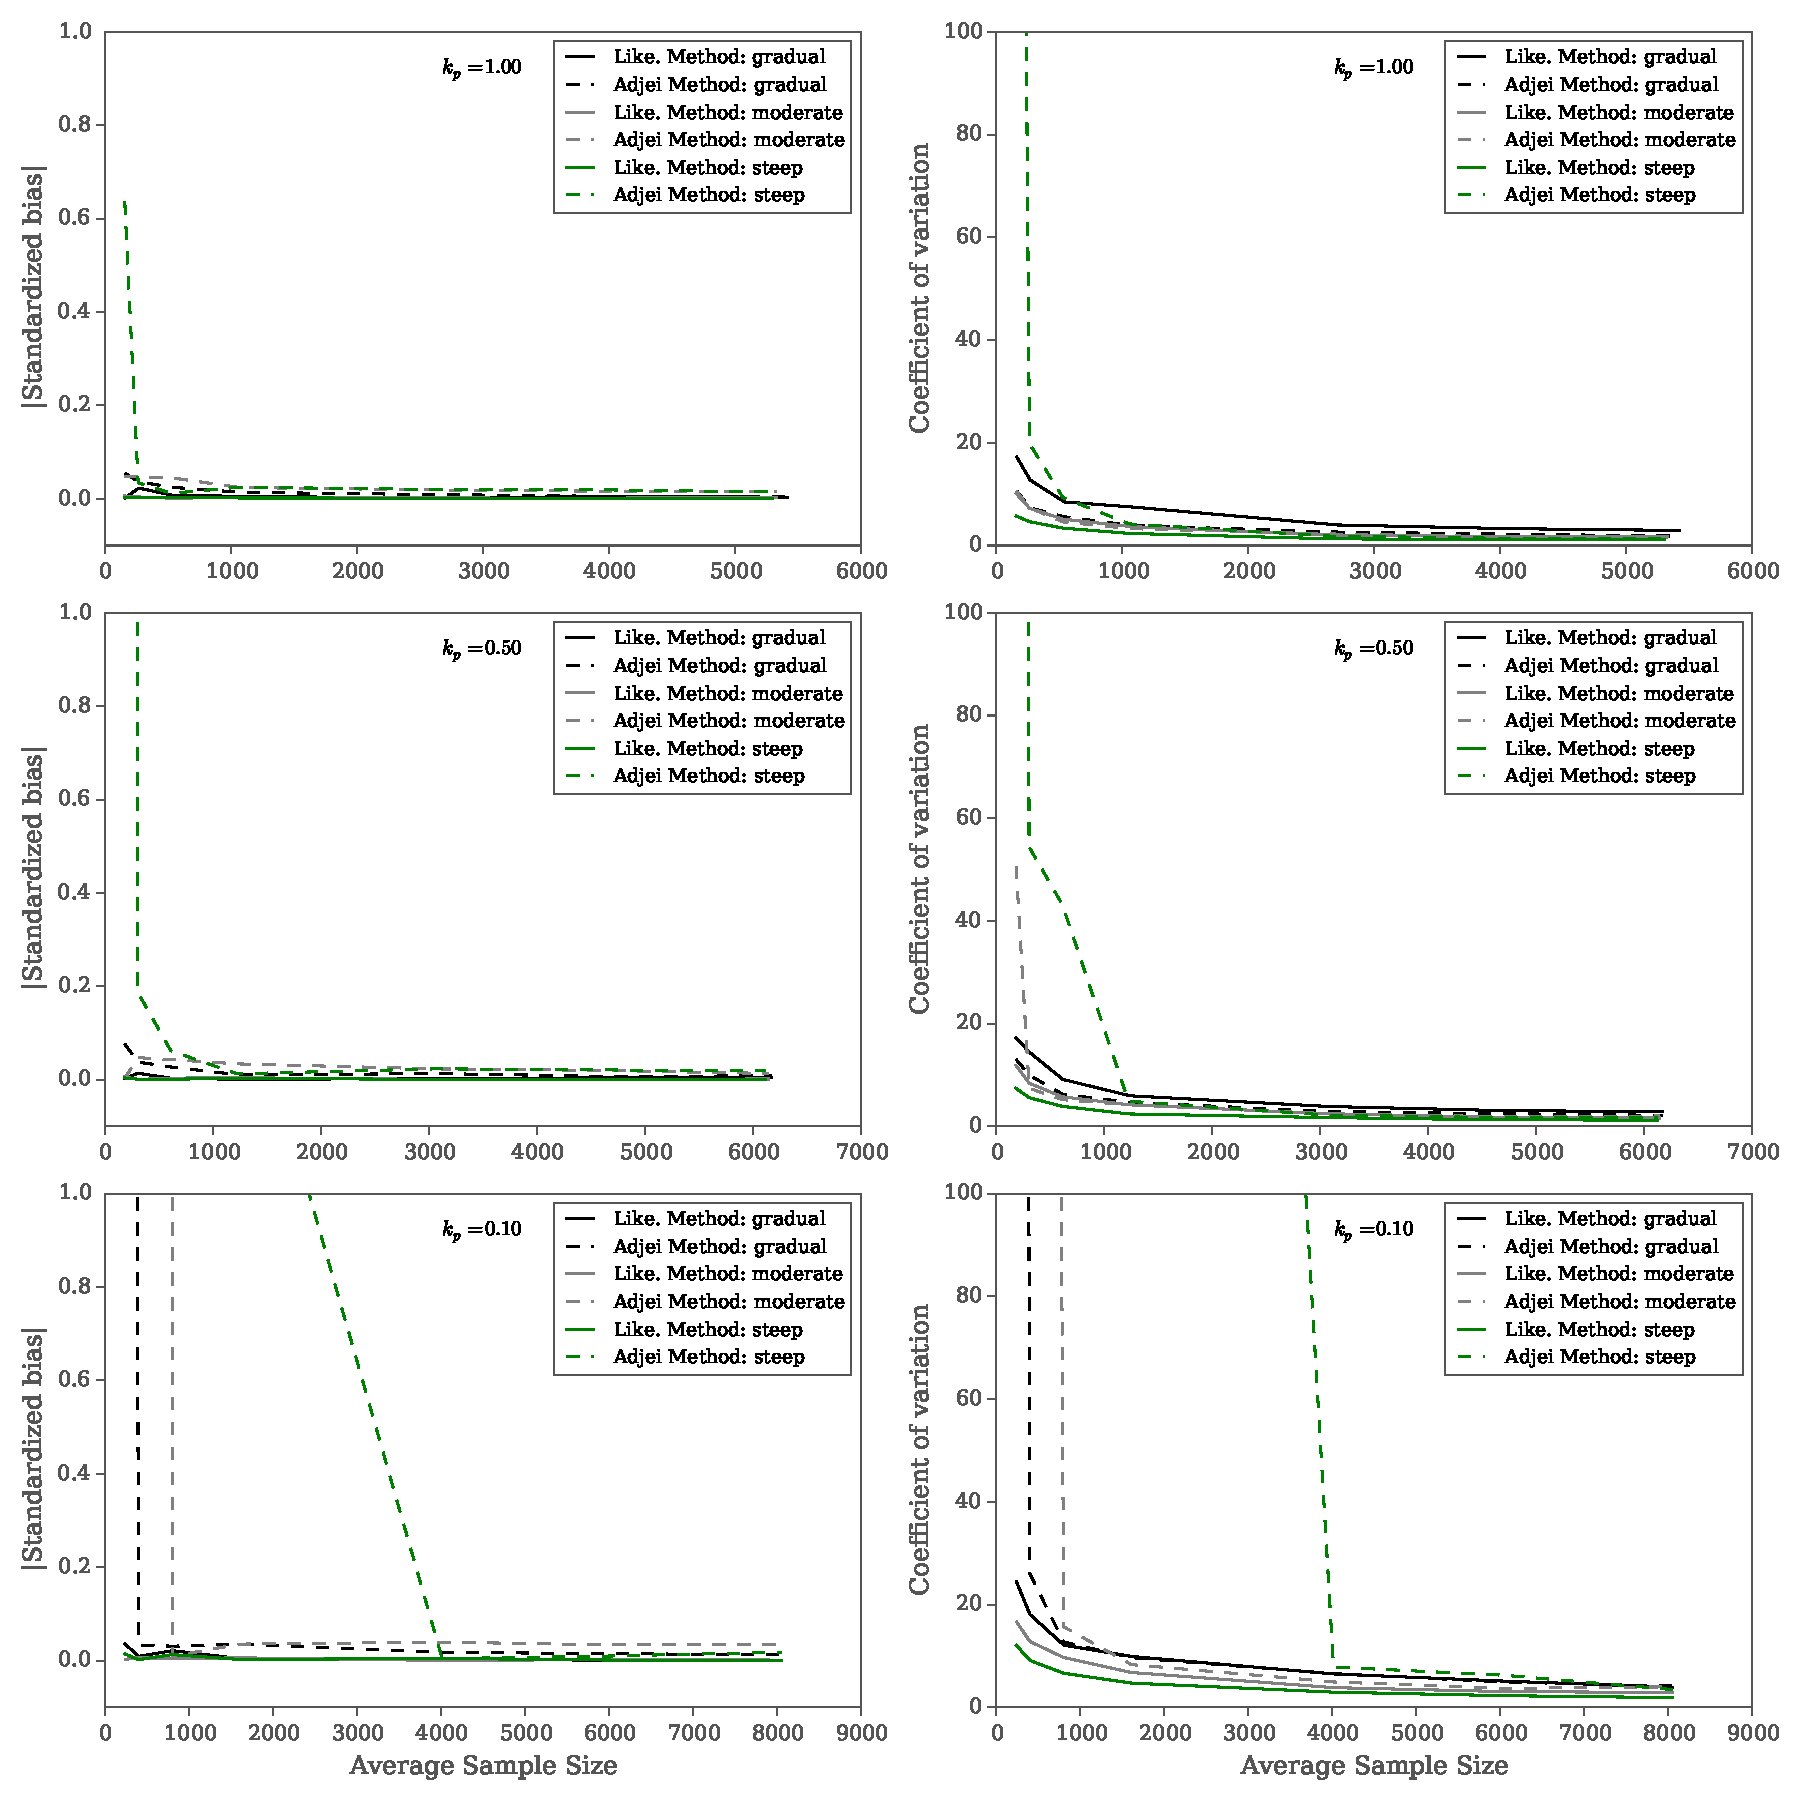
\includegraphics[width=\textwidth]{/Users/mqwilber/Repos/parasite_mortality/results/bais_prec_figure_for_ld50_mu10}

    \captionsetup{justification=centering, singlelinecheck=false}

    \caption*{\textbf{Supplementary Fig. S4}}

    %\caption{\doublespacing The bias and the precision of the Likelihood Method (black lines) and the Adjei Method (green lines) when $\mu_p = 10$ for various shapes of the host survival function and levels of aggregation $k_p$ when estimating $LD_{50}$.  The first column gives the bias of each method's $LD_{50}$ estimate over 150 simulations. The second column gives the precision of each method's $LD_{50}$ estimate over 150 simulations.}

    \label{fig:biasld50_10}

\end{figure}

\begin{figure}

    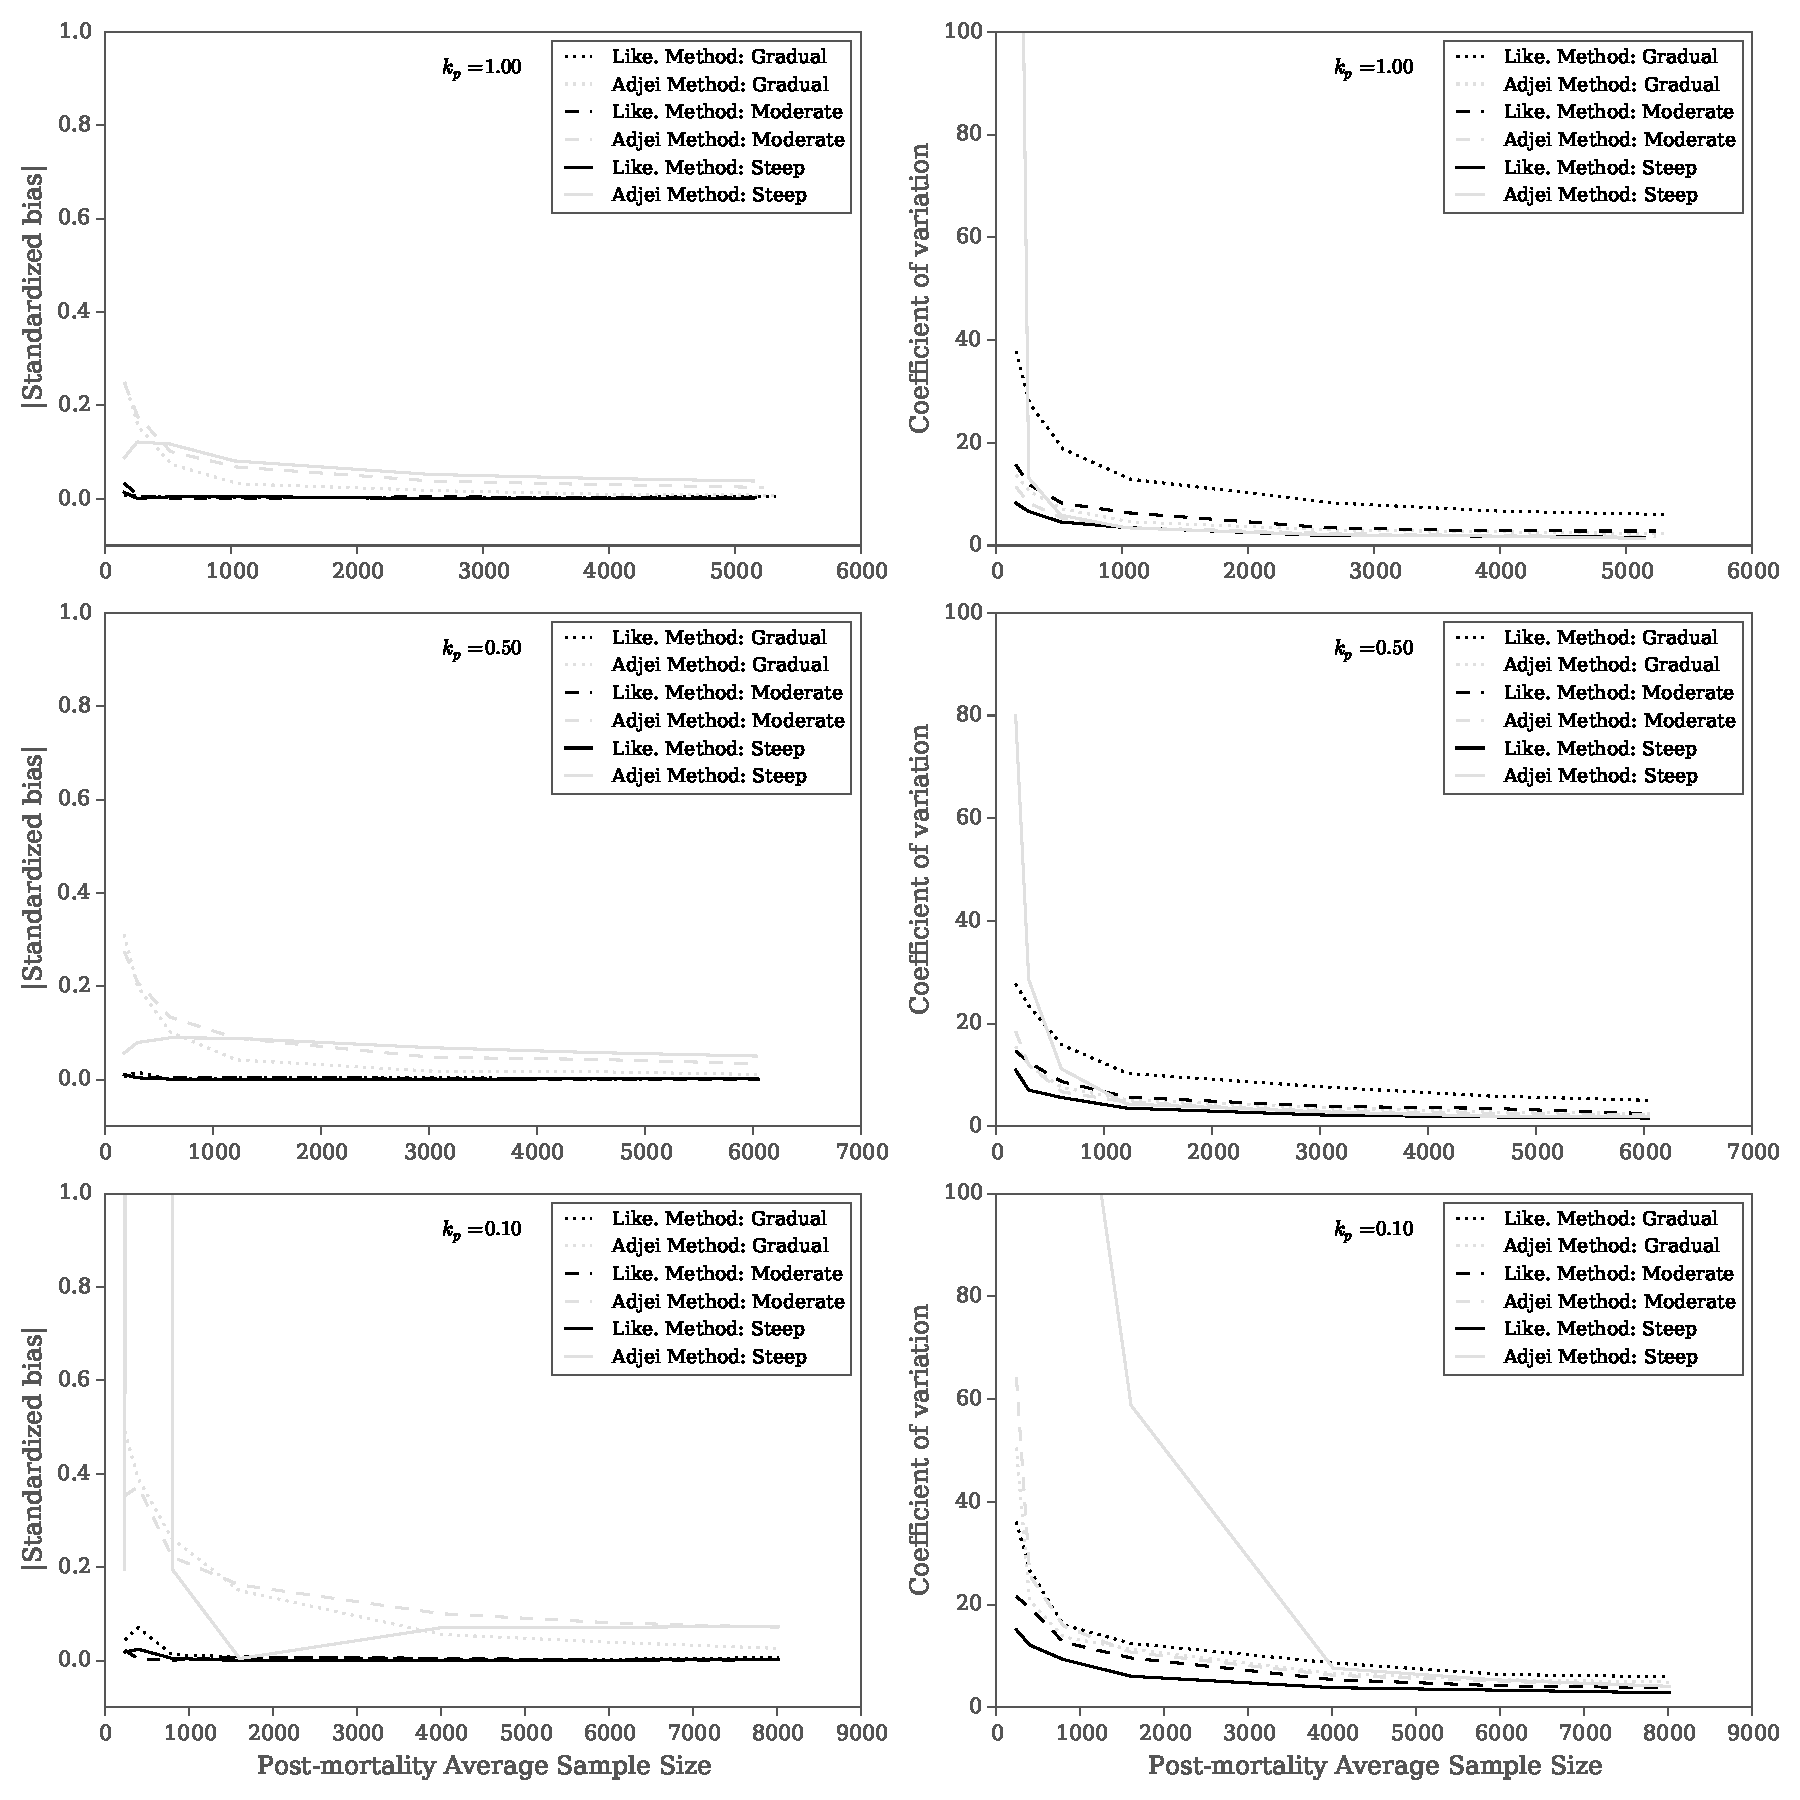
\includegraphics[width=\textwidth]{/Users/mqwilber/Repos/parasite_mortality/results/bais_prec_figure_for_ld50_mu50}

    \captionsetup{justification=centering, singlelinecheck=false}

    \caption*{\textbf{Supplementary Fig. S5}}

    %\caption{\doublespacing The bias and the precision of the Likelihood Method (black lines) and the Adjei Method (green lines) when $\mu_p = 50$ for various shapes of the host survival function and levels of aggregation $k_p$ when estimating $LD_{50}$.  The first column gives the bias of each method's $LD_{50}$ estimate over 150 simulations. The second column gives the precision of each method's $LD_{50}$ estimate over 150 simulations.}

    \label{fig:biasld50_50}

\end{figure}

\begin{figure}

    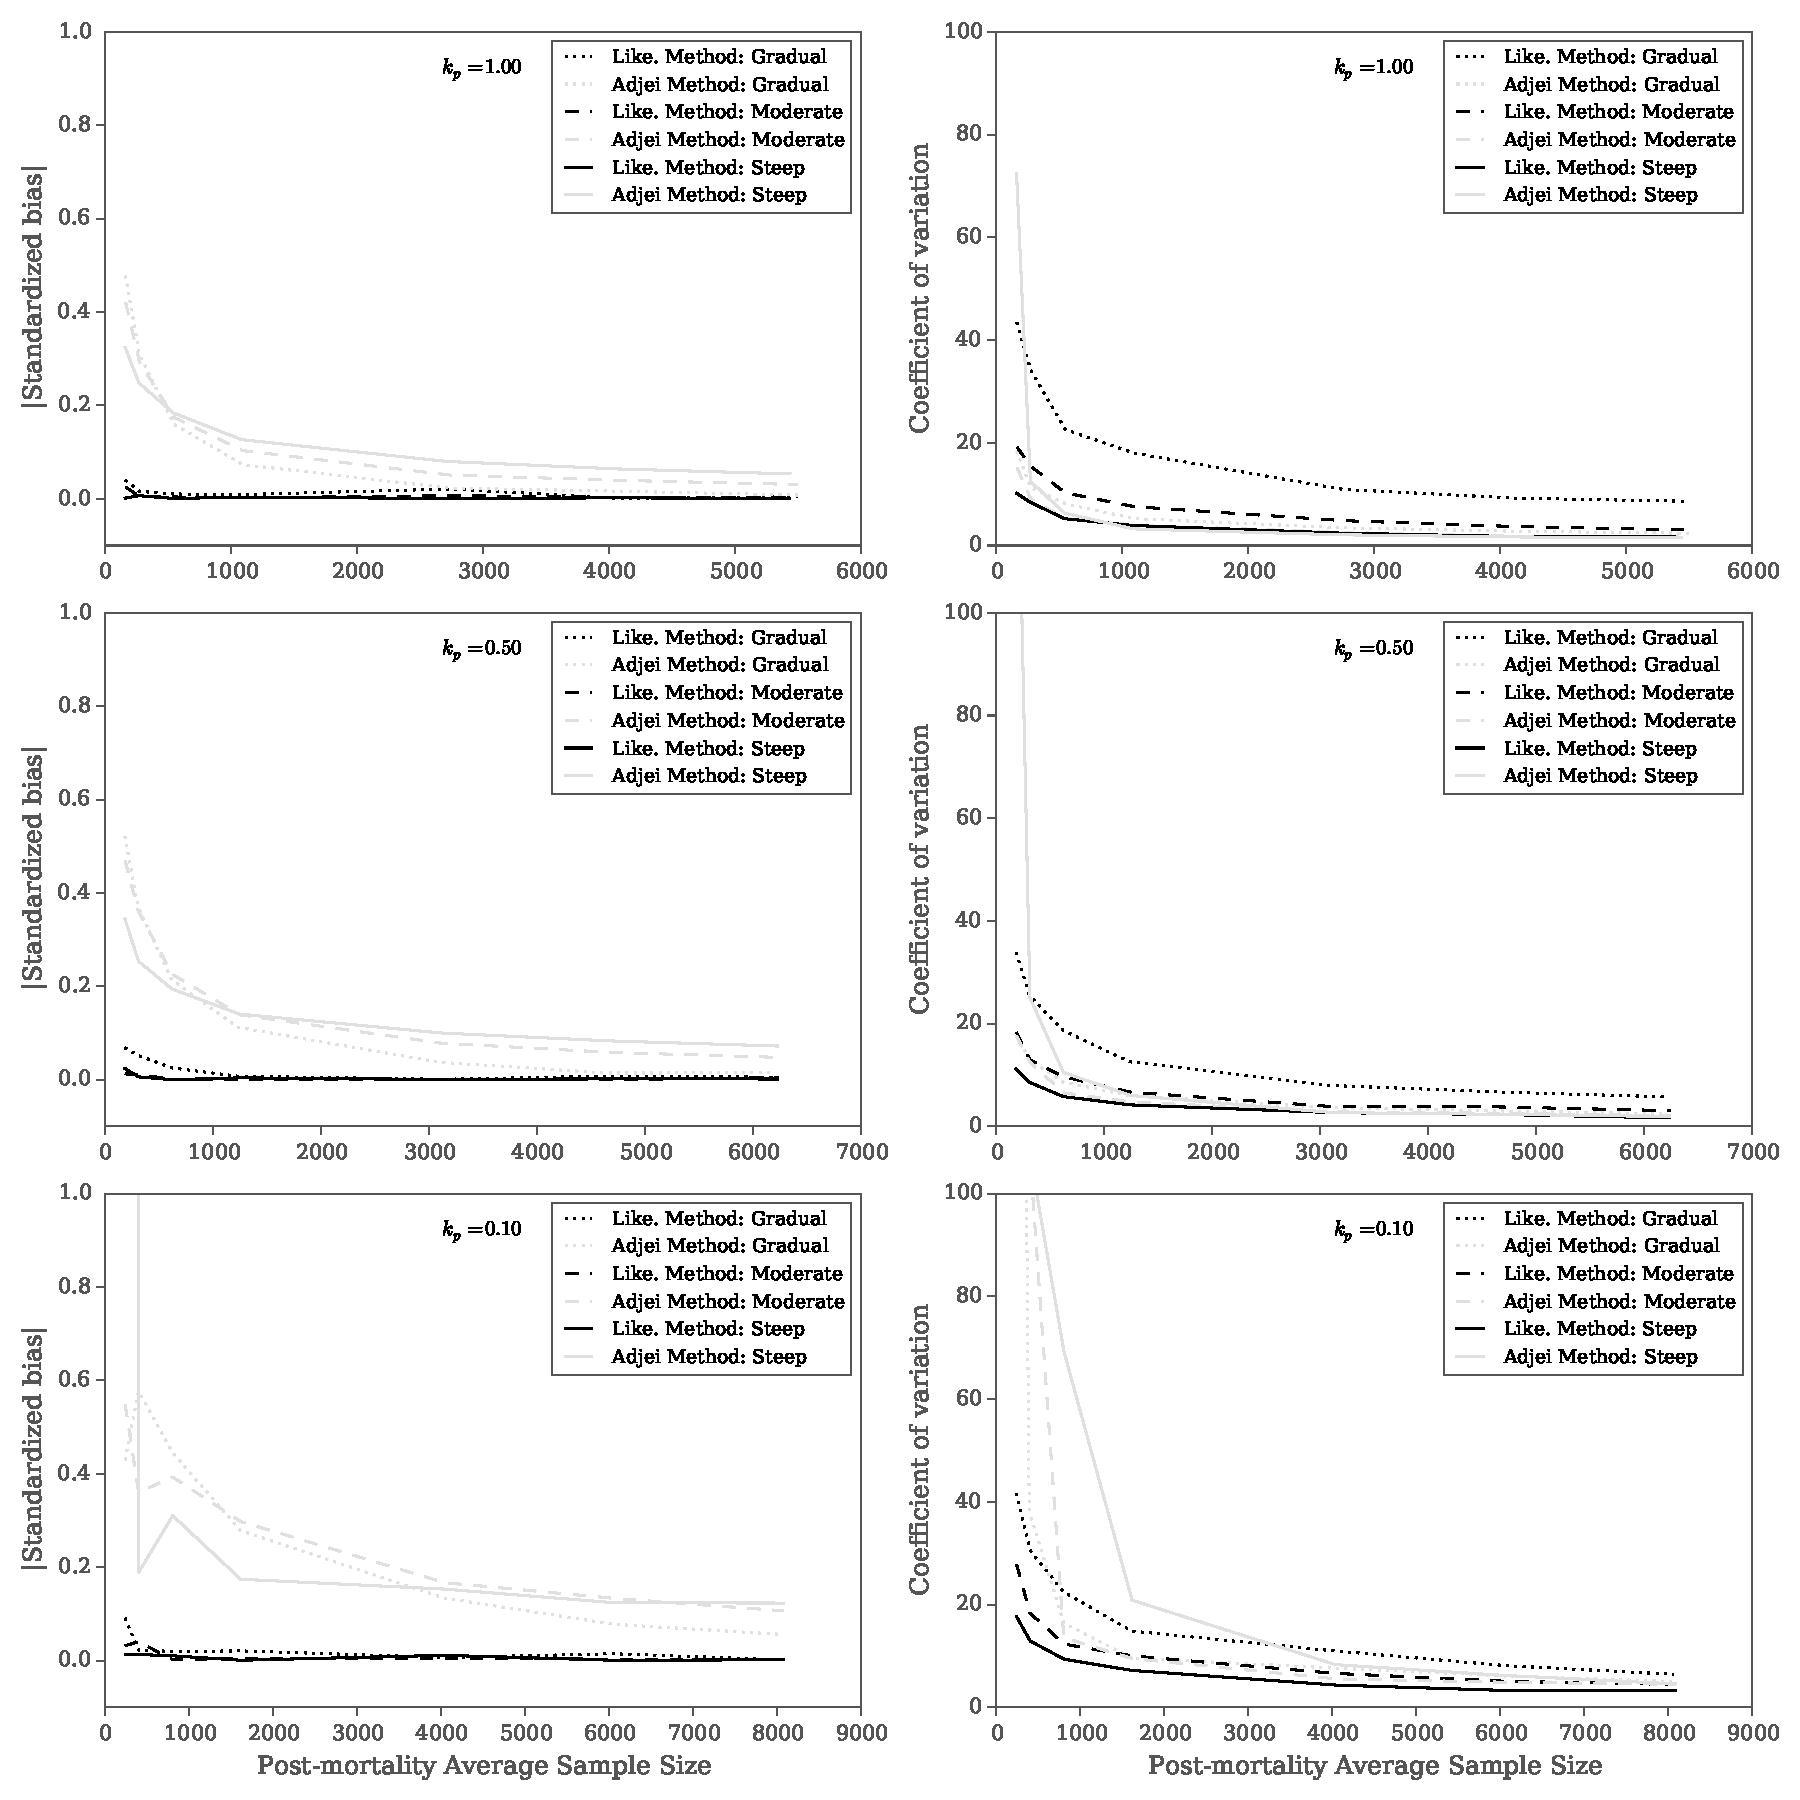
\includegraphics[width=\textwidth]{/Users/mqwilber/Repos/parasite_mortality/results/bais_prec_figure_for_ld50_mu100}

    \captionsetup{justification=centering, singlelinecheck=false}

    \caption*{\textbf{Supplementary Fig. S6}}

    %\caption{\doublespacing The bias and the precision of the Likelihood Method (black lines) and the Adjei Method (green lines) when $\mu_p = 100$ for various shapes of the host survival function and levels of aggregation $k_p$ when estimating $LD_{50}$.  The first column gives the bias of each method's $LD_{50}$ estimate over 150 simulations. The second column gives the precision of each method's $LD_{50}$ estimate over 150 simulations.}

    \label{fig:biasld50_100}

\end{figure}

\begin{figure}

    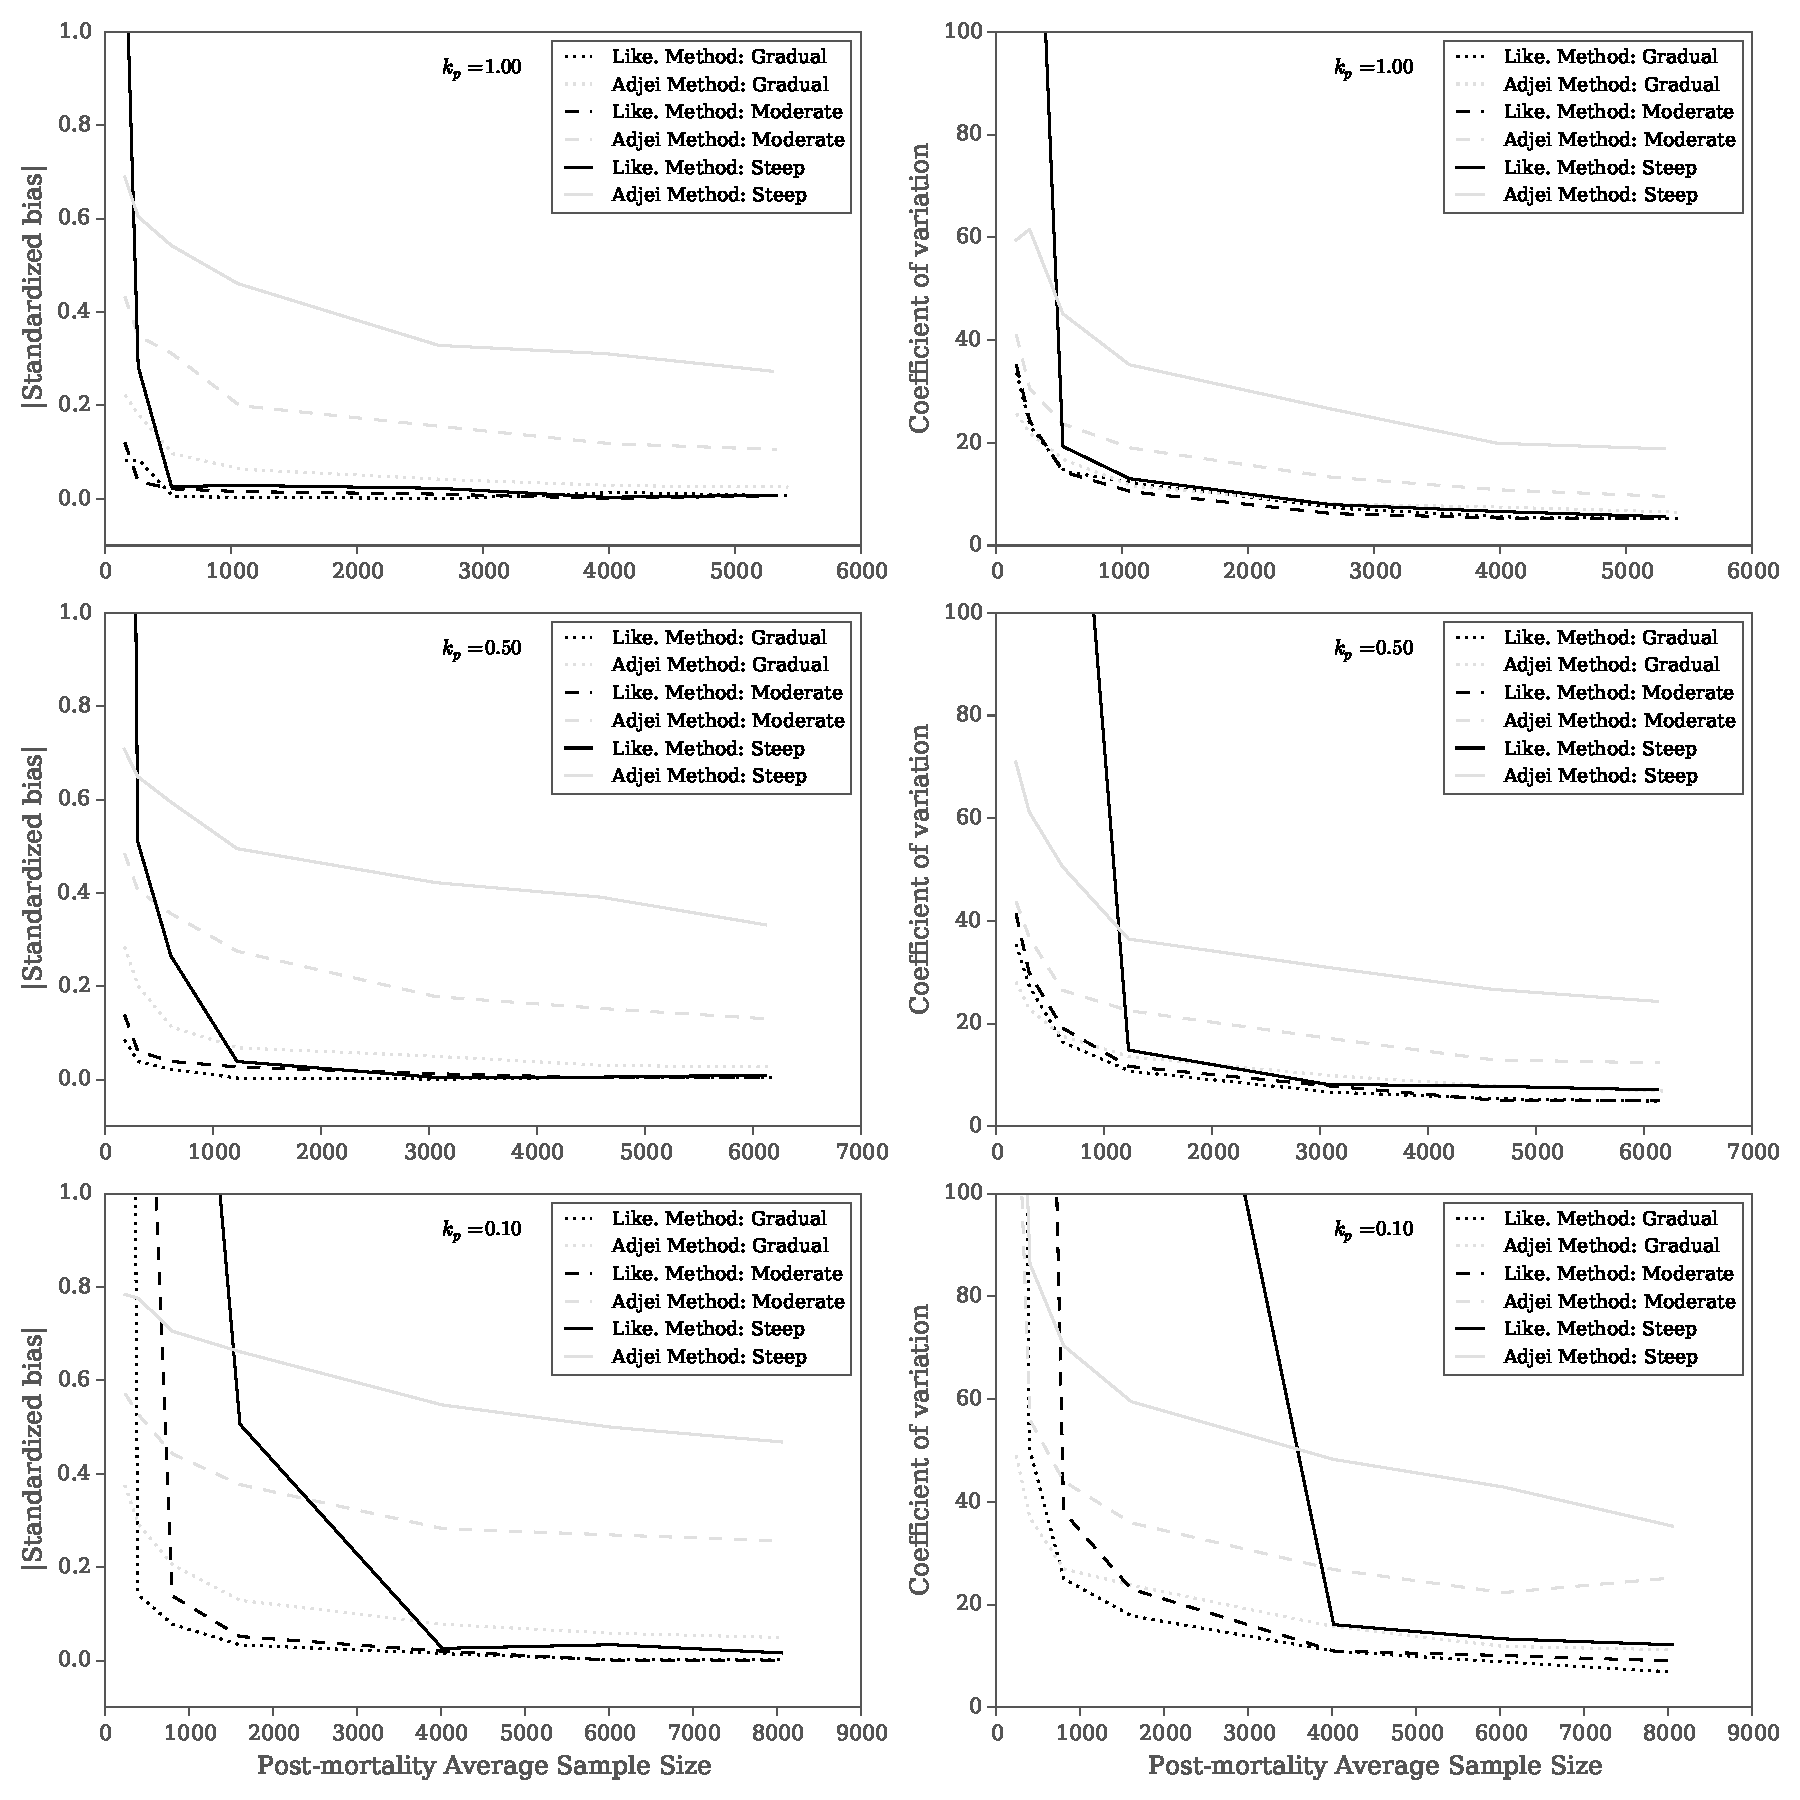
\includegraphics[width=\textwidth]{/Users/mqwilber/Repos/parasite_mortality/results/bais_prec_figure_for_a_mu10}

    \captionsetup{justification=centering, singlelinecheck=false}

    \caption*{\textbf{Supplementary Fig. S7}}

    %\caption{\doublespacing The bias and the precision of the Likelihood Method (black lines) and the Adjei Method (green lines) when $\mu_p = 10$ for various shapes of the host survival function and levels of aggregation $k_p$ when estimating the $a$ parameter of the host survival function.  The first column gives the bias of each method's $a$ estimate over 150 simulations. The second column gives the precision of each method's $a$ estimate over 150 simulations.}

    \label{fig:biasa_10}

\end{figure}

\begin{figure}

    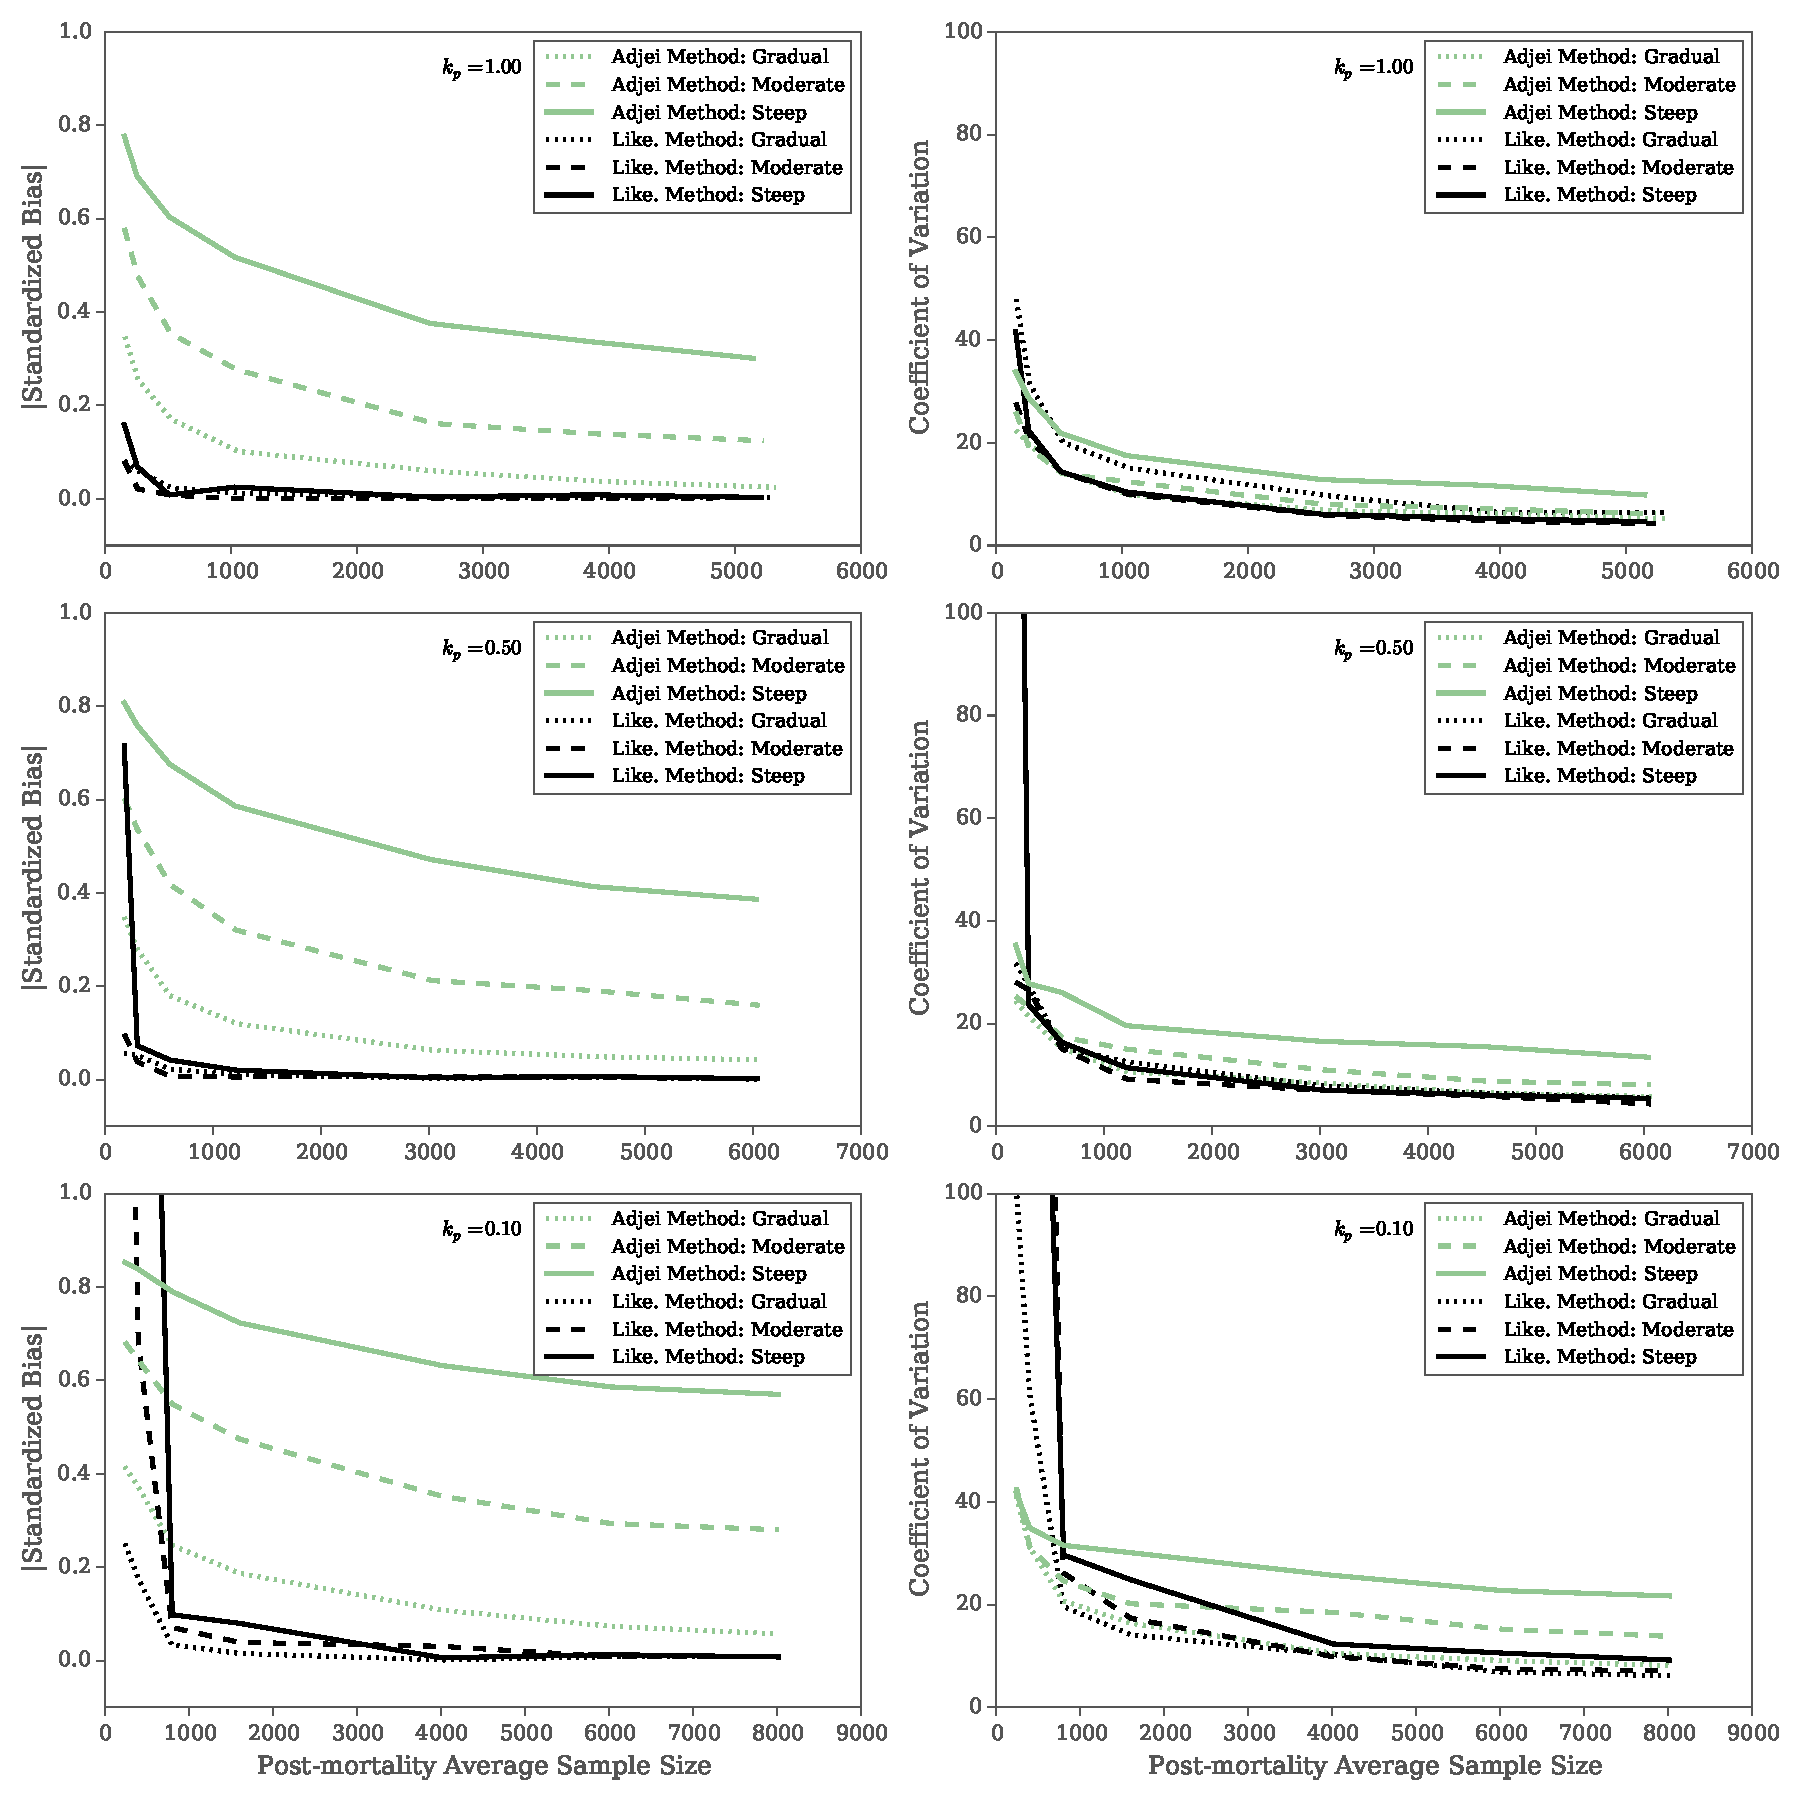
\includegraphics[width=\textwidth]{/Users/mqwilber/Repos/parasite_mortality/results/bais_prec_figure_for_a_mu50}

    \captionsetup{justification=centering, singlelinecheck=false}

    \caption*{\textbf{Supplementary Fig. S8}}

    %\caption{\doublespacing The bias and the precision of the Likelihood Method (black lines) and the Adjei Method (green lines) when $\mu_p = 50$ for various shapes of the host survival function and levels of aggregation $k_p$ when estimating the $a$ parameter of the host survival function.  The first column gives the bias of each method's $a$ estimate over 150 simulations. The second column gives the precision of each method's $a$ estimate over 150 simulations.}

    \label{fig:biasa_50}

\end{figure}

\begin{figure}

    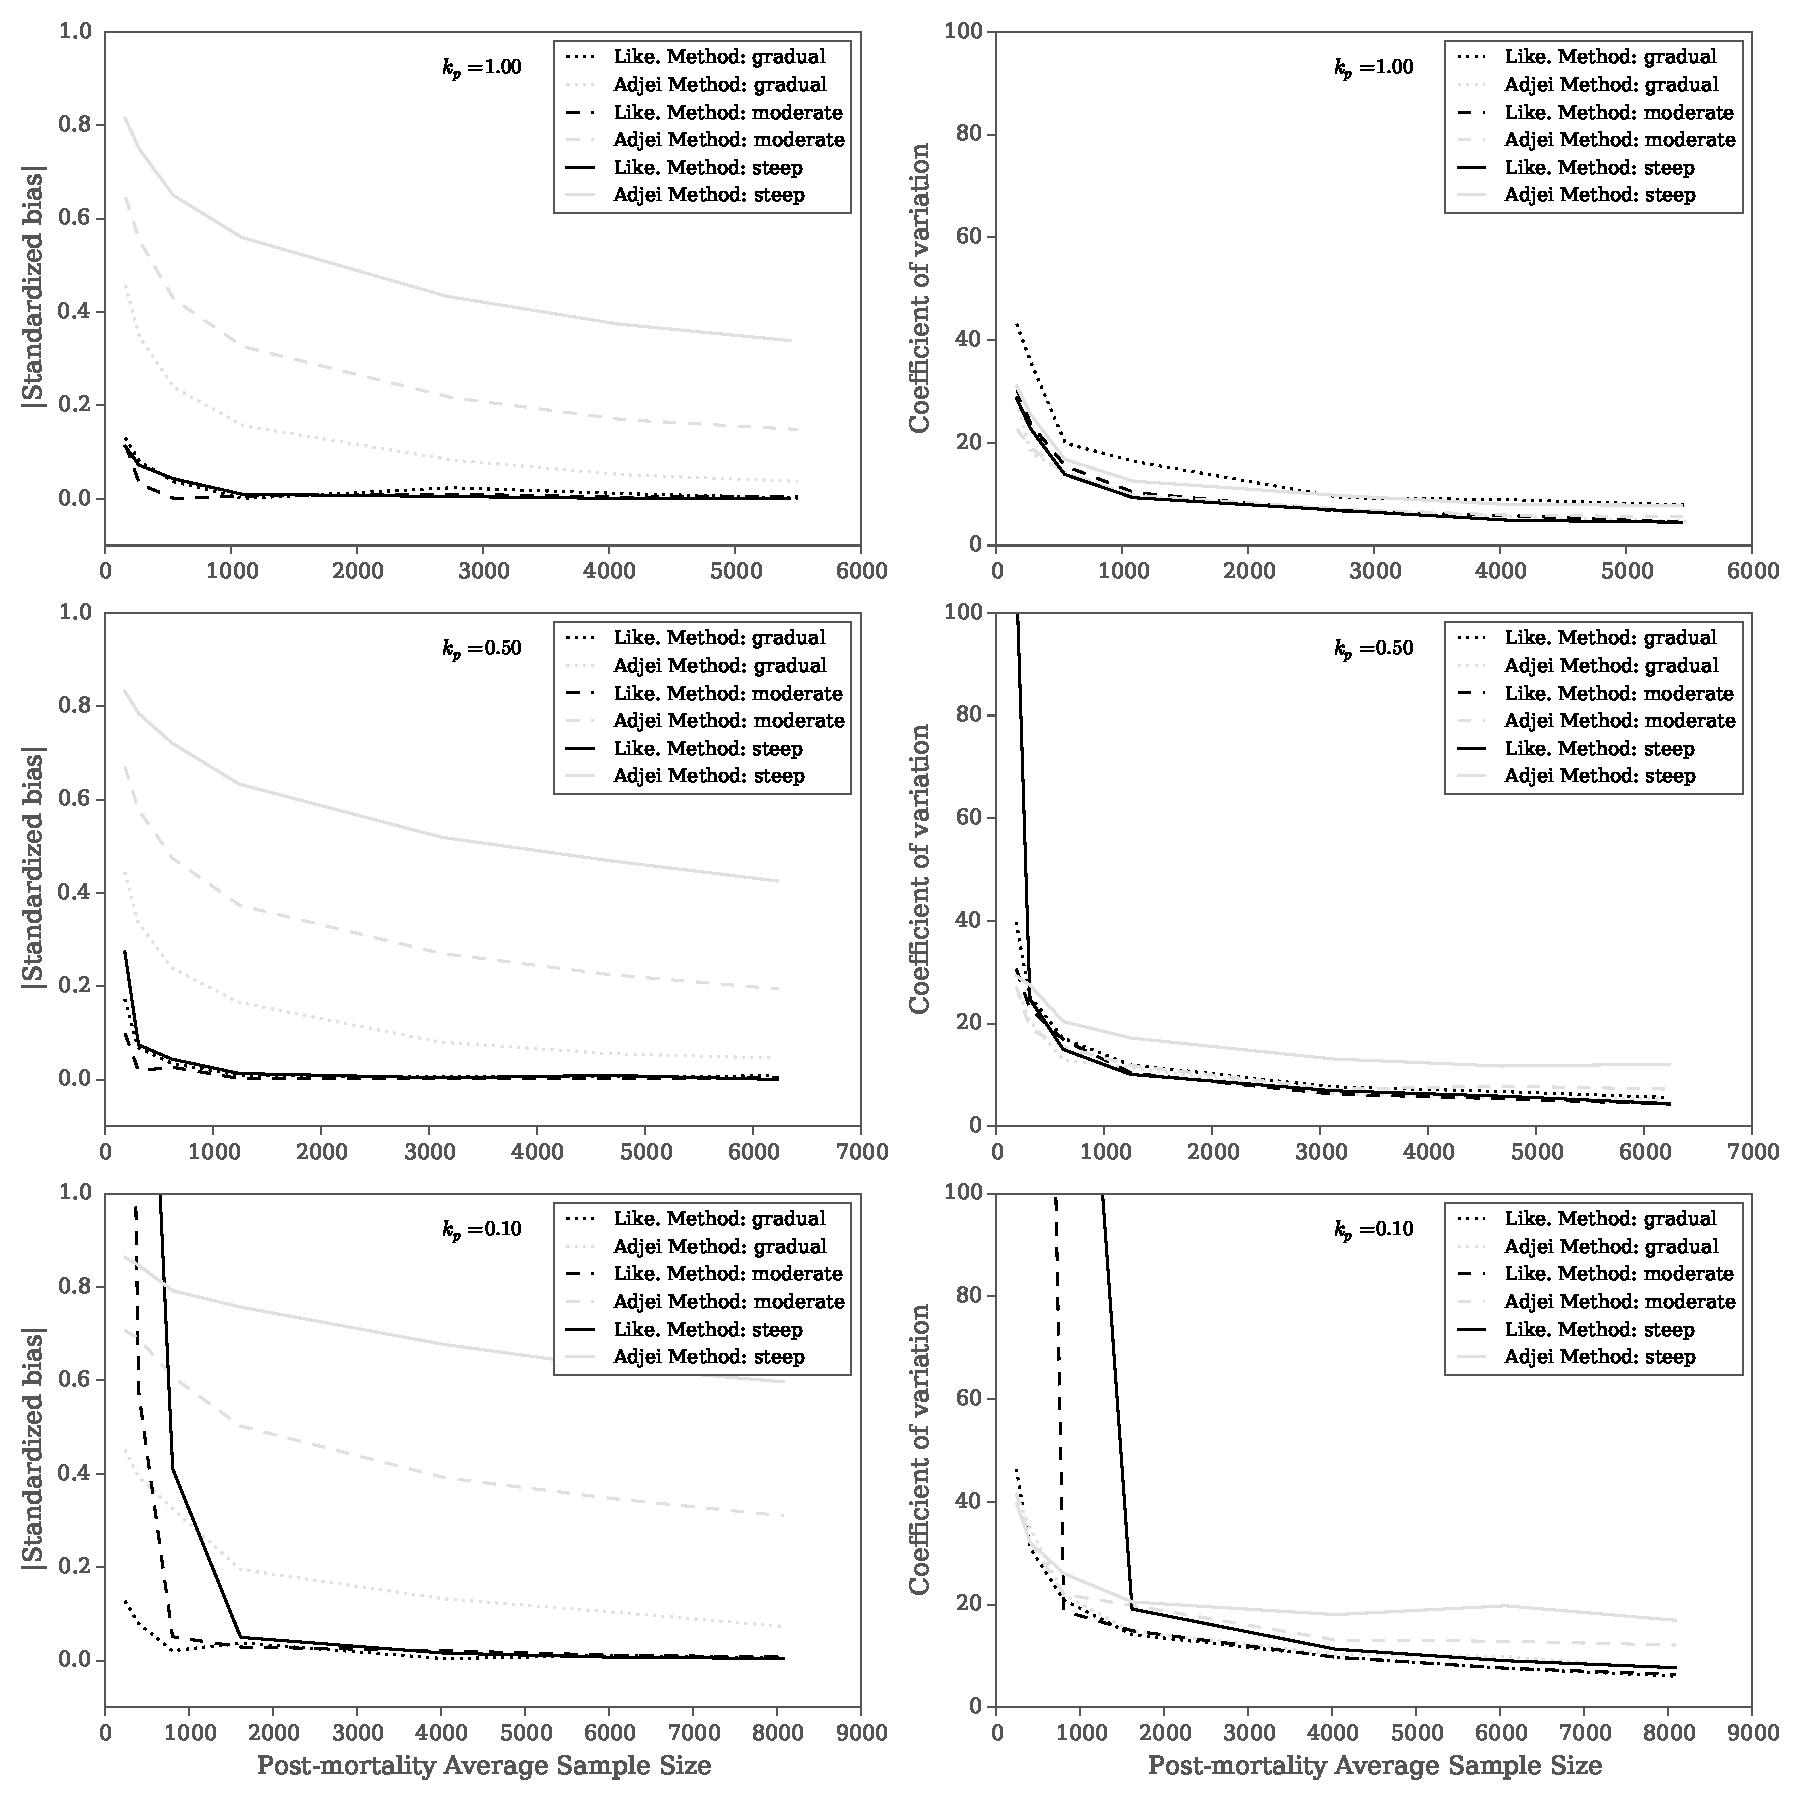
\includegraphics[width=\textwidth]{/Users/mqwilber/Repos/parasite_mortality/results/bais_prec_figure_for_a_mu100}

    \captionsetup{justification=centering, singlelinecheck=false}

    \caption*{\textbf{Supplementary Fig. S9}}

    %\caption{\doublespacing The bias and the precision of the Likelihood Method (black lines) and the Adjei Method (green lines) when $\mu_p = 100$ for various shapes of the host survival function and levels of aggregation $k_p$ when estimating the $a$ parameter of the host survival function.  The first column gives the bias of each method's $a$ estimate over 150 simulations. The second column gives the precision of each method's $a$ estimate over 150 simulations.}

    \label{fig:biasa_100}

\end{figure}

\begin{figure}

    \centering
    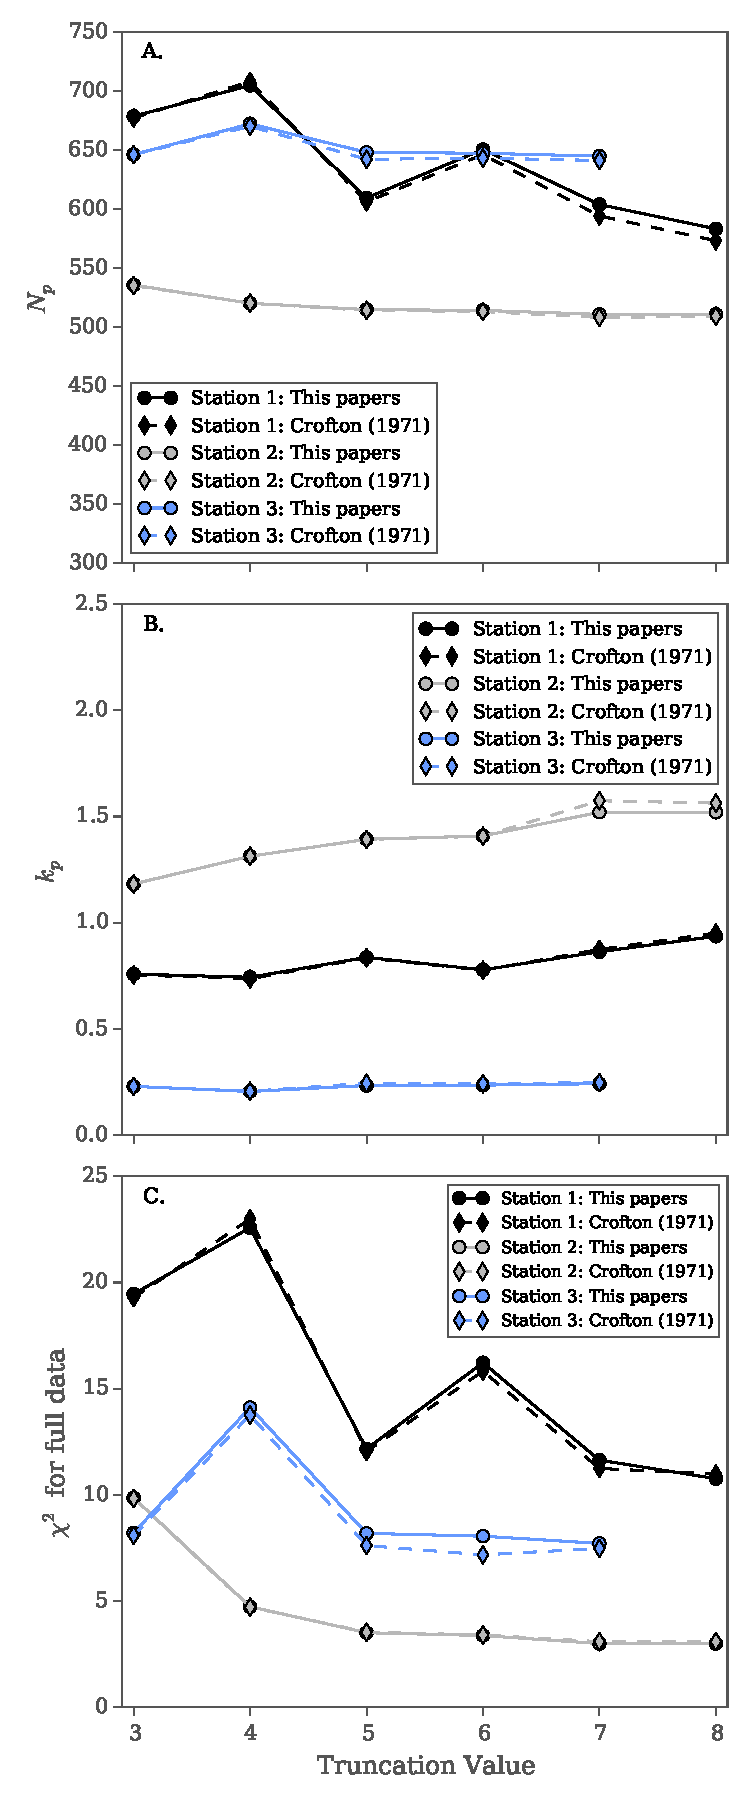
\includegraphics[width=0.5\textwidth]{/Users/mqwilber/Repos/parasite_mortality/results/compare_crofton.pdf}

    \captionsetup{justification=centering, singlelinecheck=false}

    \caption*{\textbf{Supplementary Fig. S10}}

%    \caption{\doublespacing A comparison of this paper's implementation (solid lines, circles) of the Crofton Method with the results given in \cite{Crofton1971a} (dashed lines, diamonds).  (A) compares the predicted number of hosts in a population pre-mortality ($N_p$). (B) compares the predicted parasite aggregation pre-mortality ($k_p$).  (C) compares the $\chi^2$ statistic for each implementation.  Three of the 6 stations fit by \citeauthor{Crofton1971a} are shown here and all show that our implementation gives very similar results to those given by \citeauthor{Crofton1971a}.}
    \label{fig:crof_test}

\end{figure}


\end{document}

